\fancyfoot[C]{Sandri}
\section{Motor und Motorcontroller}
	\subsection{Wahl des Motors}
		Wie schon in \ref{Motoren} Elektrische Antriebsmaschinen beschrieben, gibt es eine Vielzahl an m�glichen Maschinen zum Antrieb eines solchen Fahrzeugs. Da die Motordrehzahl hier genau geregelt werden muss eignet sich die Synchronmaschine am besten. Verwendet wird eine BLDC-Syncrhonmaschine, da diese kosteng�nstiger wie eine PMSM ist, trotzdem aber eine �hnliche Charakteristik bietet. Um eine etwas bessere Kontrolle bei langsamen Drehzahlen zu erreichen werden au�erdem Hall-Effekt-Sensoren am Motor angebracht. Der Hersteller TP-Power bietet zu einem g�nstigen Preis die M�glichkeit, Motoren auf Wunsch anzupassen und zu fertigen, gew�hlt wurder Motor TP5860 mit Hall-Effekt-Sensor er ist in folgenden Varianten verf�gbar:
		
		\begin{figure}[H]
			\centering
			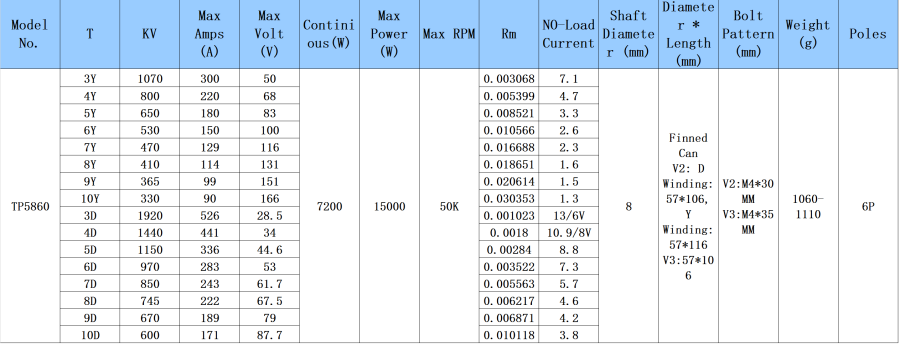
\includegraphics[scale=0.5]{./5_Elektronik/Abbildungen/TP5860}
			\caption{TP5860 Motor Konfigurationen\cite{TPPOWERUSA2024}}
		\end{figure}
		
		Die Motorkonfigurationen 8D und 4Y bilden ein gutes Gleichgewicht zwischen ben�tiger Spannung und ben�tigtem Strom, auch ist die Spannung perfekt durhc eine 16S-LiPo Konfiguration erreichbar.
		
		\subsection{Wahl des Motorcontrollers}
			Motorcontroller (auch ESCs genannt) sind in alles Gr��en, Formen und mit beliebigen Funktionen verf�gbar. Ein im Modellbau sehr bekanntes Open-Source-Projekt ist das VESC-Projekt\cite{Vedder2022}. VESCs �berzeugen durch ihre gut durchdachte Software und vielz�hlige Funktionen. Auch ist das gesamte Projekt Open-Source und kann so beliebig bearbeitet werden. Es bietet au�erdem eine Vielzahl an Schnitstellen zum Ansteuern, wie zum Beispiel UART, I2C, PWM, USB, etc. Der Hersteller FLIPSKY bietet das Model FSESC75200 Pro\cite{FLIPSKY2024} an, welches mit einer maximalen ERPM($Drehzahl * Polpaare$) von 150000, einem maximalen Strom von 300A und einer Spannung von bis 84V perfekt f�r den gew�hlten Motor geeignet ist. Es ist au�erdem sehr kosteng�nstig.
			
		\begin{figure}[H]
			\centering
			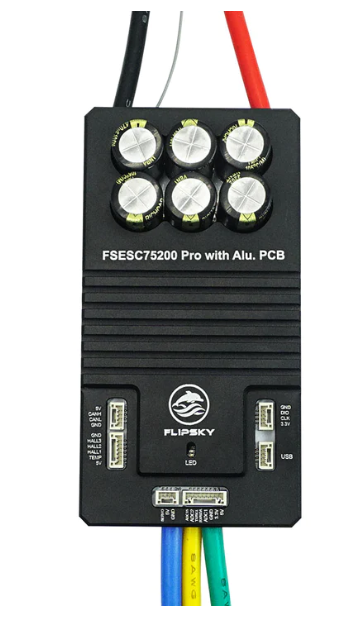
\includegraphics[scale=0.5]{./5_Elektronik/Abbildungen/VESC_0}
			\caption{TP5860 Motor\cite{FLIPSKY2024}}
		\end{figure}
			
		\subsection{Aufsetzen des Motorcontrollers}
			Als erster Schritt muss der Motor and Motorcontroller anggeschlossen werden, dazu muss man die 3 Phasen des Motors und das Hall-Effekt-Sensorkabel mit dem ESC verbinden. Danach kann man den Motor in Software konfigurieren. Das kostenlose VESC Tool erlaubt es einem, mithilfe von Laptop oder Handy, den Motorcontroller vollst�ndig auf den angeschlossenen Motor einzustellen, dies funktioniert wiefolgt:
			
			\begin{enumerate}
				
				\item Als Erstes muss der PC mit dem ESC verbunden werden, dies geht mithilfe vom AutoConnect-Knopf.
				
					\begin{figure}[H]
						\centering
						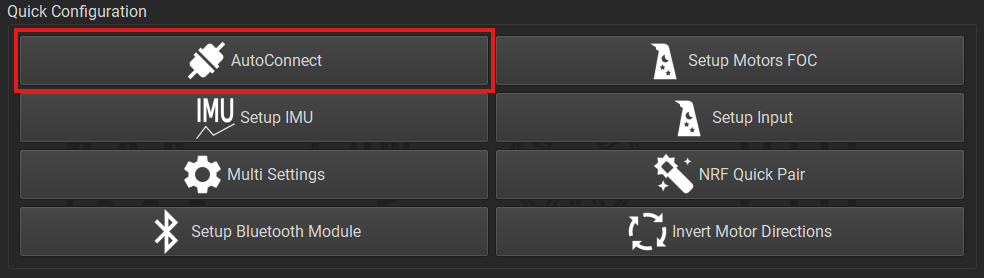
\includegraphics[scale=0.5]{./5_Elektronik/Abbildungen/VESC_16}
						\caption{VESC AutoConnect\cite{Vedder2022}}
					\end{figure}
			
				\item Als zweites kann nun der Motor konfiguriert werden, die Einstellungen daf�r k�nnen links unter dem Reiter \textbf{Motor Settings} gefunden werden. Als Erstes wird f�r die Steuerungsart FOC (Field oriented Control) gew�hlt. Hier kann auch die Drehrichtung des Motors invertiert werden.
				
					\begin{figure}[H]
						\centering
						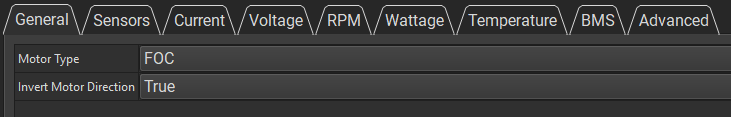
\includegraphics[scale=0.7]{./5_Elektronik/Abbildungen/VESC_2}
						\caption{VESC Steuerungstyp\cite{Vedder2022}}
					\end{figure}
					
				\item Unter dem Reiter \textbf{Sensors} wird als Sensor Hall-Sensor eingestellt, da kein Encoder verwendet wird, kann der Rest kann wie gegeben gelassen werden.	
					
					\begin{figure}[H]
						\centering
						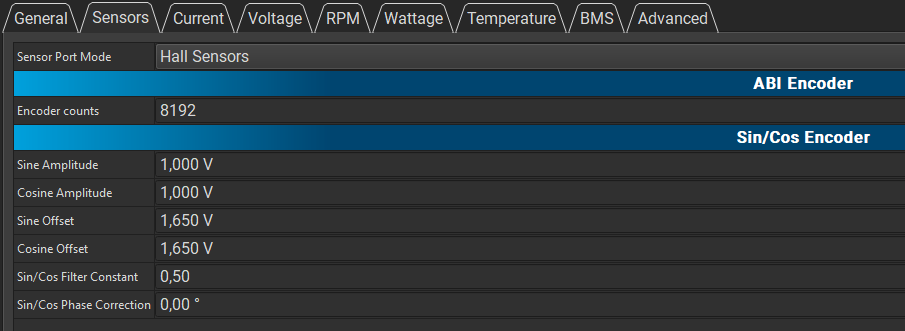
\includegraphics[scale=0.6]{./5_Elektronik/Abbildungen/VESC_3}
						\caption{VESC Sensor\cite{Vedder2022}}
					\end{figure}
					
				\item Unter dem Reiter \textbf{Current} k�nnen die Strombegrenzungen des Motors und der Batterie eingestellt werden. 	Das wichtigste ist das \textit{Absolute maximum Current} Limit, welches auf 222A gem�� dem Datenblatt vom Motor eingstellt werden sollte. \textit{Motor Current Max} und \textit{Motor Current Max Brake} werden auf 200A gesetzt, dieser Wert muss etwas unter dem absoluten Limit liegen. Das 
				
					\begin{figure}[H]
						\centering
						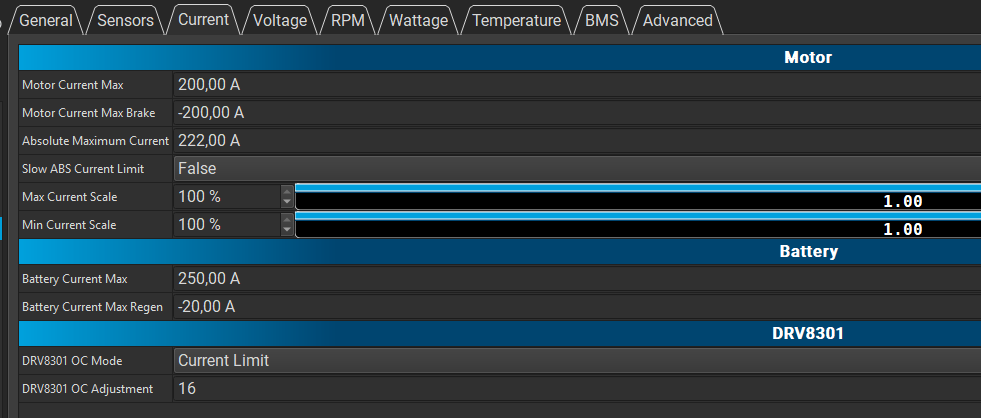
\includegraphics[scale=0.6]{./5_Elektronik/Abbildungen/VESC_4}
						\caption{VESC Current\cite{Vedder2022}}
					\end{figure}
				
				
			\end{enumerate}